\section{Methodology}
\subsection{Procedure}
The procedure used in this research is as follows:
\begin{enumerate}
	\item Use a mutation testing tool (PIT) to produce faulty program and run it against master test suite. Get mutant status for every test case.
	\item Generate a large number of test suites by randomly selecting tests cases from master test suite, until the test suite reaches its pre-defined size.
	\item For each test suite:
	\begin{itemize}
		\item Measure coverage criteria (CodeCover) for different test suites.
		\item Determine effectiveness of different test suites using mutation information and coverage criteria.
	\end{itemize}
	\item Analyse correlation between different coverage criteria and effectiveness.
\end{enumerate}

\subsection{Subjects under test}
The original paper used five following subject programs: 
\begin{enumerate}
	\item Apache POI~\cite{apachepoi}: a Java API for Microsoft Documents
	\item Closure~\cite{closure}: a tool for making JavaScript download and run faster.
	\item HSQLDB~\cite{hsqldb}: a Java SQL relational database.
	\item JfreeChart~\cite{jfreechart}: a Java chart library for users to display professional quality charts.
	\item Joda Time~\cite{jodatime}: A replacement for Java time and date class
\end{enumerate}

These five subjects are selected on purpose using the following criteria:
\begin{enumerate}
	\item The program needs to be large enough to have more than 100,000 SLOC;
	\item It needs to be an actively developed Java program;
	\item It contains at least 1000 test cases;
	\item The project needs to use Ant as its build system;
	\item The project uses JUnit as a test harness.
\end{enumerate}

However no versions or git hashes of subject programs were given in the original paper or in its artefact page. As the original paper was published in 2014, various number of test subjects versions between 2012 to 2014 were examined with different PIT versions, but there was no result that was close enough to what was reported in the original paper. Figure~\ref{fig:jodamutant} and figure~\ref{fig:jodakilled} are examples of different versions of Joda Time running against PIT version 1.0.0. We contacted authors of the original paper, and acquired their project repository.


\begin{figure}[h]
	\centering
	\begin{minipage}{0.4\textwidth}
		\centering
		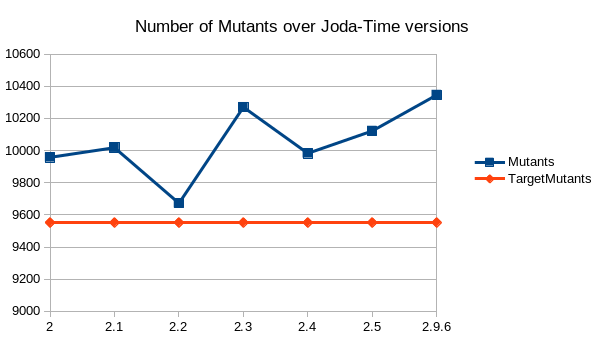
\includegraphics[width=\textwidth]{Figure/joda_mutant.png}
		\caption{Joda Time total mutants}
		\label{fig:jodamutant}
	\end{minipage} %
	\begin{minipage}{0.4\textwidth}
		\centering
		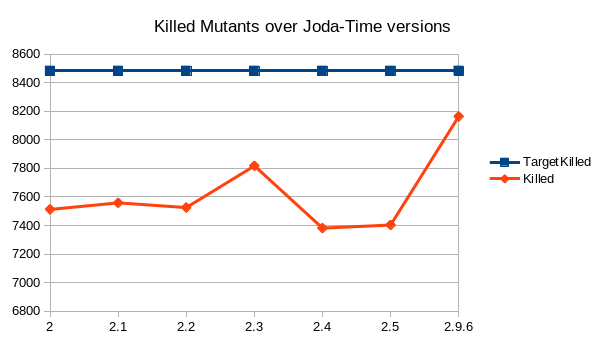
\includegraphics[width=\textwidth]{Figure/joda_kill.png}
		\caption{Joda Time killed mutants}
		\label{fig:jodakilled}
	\end{minipage}
\end{figure}

There are some environment settings need to be adjusted locally. Mutation testing tool PIT used for this project requires green test suite, which means all tests must pass. During my replication, some projects provided by the author could not compile or did not pass all tests. The first Java compiler used in the replication was Java 8, but non of the projects passed all tests. HSQLDB, JfreeChart, Joda Time worked with no errors using Java 7. According to ant build system, recommanded Java compiler for Closure was Java 6, but non of the compiler version complied it successfully. For Apache POI, Java 6 and 7 compilation was successful but resulted failing tests.

There was no command to exclude failing tests in author's repository, and the report log suggests the Apache POI and Closure were working correctly. I suspected that authors made some change after they got result for Apache POI and Closure. So I downloaded source code from GitHub according to author's repository. Table~\ref{tab:sut} is a summary of projects and compiler version. Java 7 was selected as final replication compiler.


\begin{table}[h]
	\caption{Java Compiler Setting}
	\label{tab:sut}
	\begin{minipage}{\columnwidth}
		\begin{center}
			\begin{tabular}{|l|l|c|c|c|c|c|c|}
				\hline
				&&\multicolumn{2}{|c|}{Java 6}&\multicolumn{2}{|c|}{Java 7}&\multicolumn{2}{|c|}{Java 8}\\
				\hline
				Project & Version & Compile & Test & Compile & Test & Compile & Test \\
				\hline
				Apache POI & 3.9(author) & Success & Fail & Success & Fail & Success & Fail \\
				& 3.9(GitHub) & Success & Success& Success& Success & Success& Fail \\
				\hline
				Closure& 20130227(author) & Fail & Fail & Fail & Fail & Fail & Fail \\
				&20130227(GitHub) & Success & Success & Success & Success & Success & Fail \\
				\hline
				HSQLDB & 2.2.8 & Success & Success & Success & Success & Success & Fail \\
				\hline
				JfreeChart & 1.0.8 & Success & Success & Success & Success & Success & Fail \\
				\hline
				Joda Time & 2.0 & Success & Success & Success & Success & Success & Fail \\
				\hline
			\end{tabular}
		\end{center}
		\bigskip
	\end{minipage}
\end{table}

The final environment settings used in this replication study are:
\begin{itemize}
	\item Operating System: Ubuntu 14.04.5 LTS;
	\item Java Compiler: 1.7.0\_u131;
	\item ant build system: 1.9.3;
	\item JUnit: 3.8 for compiling projects, 4.10 for running PIT;
	
Other systems should work, as long as using Java compiler 7, ant version greater than 1.8; and having JUnit 3 and JUnit 4  at the same time.
\end{itemize}


\subsection{Mutation Testing}
\label{subsec:mutationTesting}
Mutation testing of the program was conducted using an automated mutilation testing tool PIT~\cite{pit}, which is one of the most widely used open source Java mutation testing system. Version of PIT used for the original paper was 0.30-SNAPSHOT. PIT run tests against automatically generated mutants. Firstly it performs statement coverage for the tests, then use coverage information to pick test cases targeting a particular mutant.

For a mutant, PIT reports one of the following result status:
\begin{itemize}
	\item Killed: mutant has been killed by the test suite.
	\item Survived: mutants have at lease one test case execute it but survived.
	\item No coverage: mutants lived because no test case executed the line of code where the mutant was created. 
	\item Time out: the mutants causes an infinite loop, for example mutate loop counter in a for loop.
	\item Non viable: the mutant is invalid and can not be loaded by the Java Virtual Machine (JVM).
	\item Memory error: the mutation requires more memory to be used by system.
	\item Run error: there is something wrong when running the mutant.	
\end{itemize}

Under normal circumstances, there should be no non viable mutants or errors.

Although author did not mention in the paper, she has made some modification to PIT. For the original PIT, if a mutant is killed by a test case, the test case is logged, then PIT moves to next mutant. As a result, PIT firstly provides a boolean information of whether mutant is killed, then only the first test case killed the mutant was reported. The research wanted information about all test cases that detect a mutant, so modification is required. For the modified PIT, a mutant run against all possible test cases target it, PIT moves to next mutant until covered test cases are executed, and result for every test case and its corresponding mutant is logged in a log file. The modification is valid for 4 out of 5 subjects, but generated different results for HSQLDB compare to PIT default report. This will be discussed in more detail in section~\ref{subsec:resultPIT}

\subsection{Test suite generation}
For each subject program, Java’s reflection API was used to identify all of the no-argument test methods in the program’s master test suite. Then new test suites were generated size by randomly selecting a subset of master suite without replacement until predefined size was reached.

Size of the test suite follow the pattern: 3, 10, 30, 100, up to the largest number follow this pattern and less than the total test cases for the project. The largest suite used for Apache POI and JFreeChart was 1000, and for Closure and Joda Time was 3000.

But in replication, when we selected random subsets of the project master test suites, some of the random test suites fail to pass unit test, even though they pass in the master test suite. We contacted author for this problem, and got reply that there were failing tests excluded, but we can not find the list of excluded tests in the archive provided.

we investigated the chance of appearance of failing random test suite. And we found that it happened rarely as shown in Table~\ref{tab:failtest}. Running random test suite analysis is very time consuming, finding all failing test combination is impossible for the given time. So we decided to ignore the failing methods as they do not have significant influence on results.

\begin{table}[h]
	\caption{Number of failing tests appeared in random test suite selection}
	\label{tab:failtest}
	\begin{minipage}{\columnwidth}
		\begin{center}
			\begin{tabular}{c|c|c|c|c}
				\hline
				Size & Apache POI & Closure & JFreeChart & Joda Time \\
				\hline
				3 & - & - & - & - \\
				10 & - & - & - & 1 \\
				30 & - & - & 1 & - \\
				100 & - & - & 1 & - \\
				300 & - & - & - & 1 \\
				1000 & - & - & - & - \\
				3000 & - & - & - & - \\
				\hline
			\end{tabular}
		\end{center}
		\bigskip
	\end{minipage}
\end{table}

\subsection{Coverage Measurement}
Coverage criteria are measured using an open source Java coverage analysis tool CodeCover~\cite{codecover}. Statement, decision and modified condition types are used in the project.

Statement coverage is measured for the following statement type:
\begin{itemize}
	\item assignments and method calls
	\item variable and member declaration with an assignment
	\item break
	\item continue
	\item return
	\item throw
	\item empty statements
\end{itemize}

All condition statements such as if and for are not considered for statement coverage.

Decision branches are measured for the branches:
	\begin{itemize}
		\item if-else statements: one branch for if and another for else
		\item switch-case statements: a branch for each case and one for default
		\item try-catch statements: one bran for every catch, one branch for exceptions not in catch cases and one branch for successful execution.
	\end{itemize}

MCC coverage consider the boolean expressions in:
	\begin{itemize}
		\item if
		\item for
		\item while and do...while
	\end{itemize}
Boolean expressions not in decision or looping statements are ignored, such as assignments.

\subsection{Effectiveness}
\label{subsec:effectiveness}
As mentioned in Section~\ref{sec:related}, there are two effectiveness introduced in this paper: raw effectiveness measurement and normalised effectiveness measurement. Author did not give mathematical expression for two effectiveness.

Raw effectiveness is the number of killed mutants of a test suite divided by the number of killed mutants of master test suite. For a test suite t, master suite T and program P, raw effectiveness should be:
\[\textit{rawEffectiveness} = \frac{\#\textit{killedMutants(t,P)}}{\#\textit{killedMutants(T,P)}}\]

For a test suite normalised effectiveness and is calculated by killed mutants of this suite over covered non-equivalent mutants of the same suite. Directly from authors' definiation we have the expression, for a test suite t and program P:
\[\textit{normalisedEffectiveness} = \frac{\#\textit{killedMutants(t,P)}}{\#\textit{coveredNon-equivalentMutants(t,P)}}\]

The number of covered non-equivalent mutants is the maximum mutants a test suite can possibly detect. A mutant can have three status for a particular test suite: covered and killed by test cases in this test suite, covered but not killed by this test suite but killed by test cases outside this test suite and surviving or equivalent. Covered non-equivalent mutants are total mutants covered taking away surviving mutants. So the final equation of normalised effectiveness for a test suite t and program P is:
\[\textit{normalisedEffectiveness} = \frac{\#\textit{killedMutants(t,P)}}{\#\textit{totalCoveredMutants(t,P)} - \#\textit{equivalentMutants(t,P)}}\]

\subsection{Correlation Measurement}

Kendall’s $\tau$ correlation coefficient is used in the original paper. Kendall’s $\tau$ is similar to the more common Pearson coefficient but does not assume that the variables are linearly related or that they are normally distributed. Rather, it measures how well an arbitrary monotonic function could fit the data. Kendall’s $\tau$ was used to avoid unnecessary assumptions.

The original paper used the Guildford scale~\cite{guilford1942fundamental} for verbal description, in which correlations with absolute value less than 0.4 are described as “low”, 0.4 to 0.7 as “moderate”, 0.7 to 0.9 as “high”, and over 0.9 as “very high”.